\documentclass[11pt,a4paper]{article}

% ---- Packages ----
\usepackage[utf8]{inputenc}
\usepackage[T1]{fontenc}
\usepackage[english]{babel}

\usepackage[margin=1.1in]{geometry}
\usepackage{amsmath, amssymb, amsthm, mathtools}
\usepackage{booktabs, array}
\usepackage{enumitem}
\usepackage{xcolor}
\usepackage{graphicx}
\usepackage{epigraph}
\usepackage{csquotes}
\usepackage{tikz}
\usetikzlibrary{arrows.meta, positioning, shapes.geometric, shapes.misc,
                fit, calc, backgrounds, decorations.pathreplacing,
                patterns, matrix}
\usepackage{pgfplots}
\pgfplotsset{compat=1.18}

\usepackage[colorlinks=true, linkcolor=black!70!blue,
            citecolor=black!70!blue, urlcolor=black!40!blue]{hyperref}

% ---- Theorem environments ----
\theoremstyle{definition}
\newtheorem{definition}{Definition}[section]
\newtheorem{example}[definition]{Example}

\theoremstyle{remark}
\newtheorem*{remark}{Remark}
\newtheorem*{aside}{Aside}

\theoremstyle{plain}
\newtheorem{proposition}[definition]{Proposition}

% ---- Epigraph style ----
\setlength{\epigraphwidth}{0.6\textwidth}
\renewcommand{\epigraphflush}{flushright}
\renewcommand{\textflush}{flushright}
\renewcommand{\epigraphsize}{\small\itshape}

% ---- Small conveniences ----
\newcommand{\todo}[1]{\textcolor{red!70!black}{\textbf{[TODO: #1]}}}
\newcommand{\MFU}{\mathrm{MFU}}
\newcommand{\HFU}{\mathrm{HFU}}
\newcommand{\FPN}[1]{\textrm{FP#1}}
\DeclareMathOperator*{\argmin}{arg\,min}

% ---- Title ----
\title{\textbf{Efficient Deep Learning Systems} \\[0.3em]
       \large Lecture 2 --- Optimizing Training Pipelines: \\
       Performance Indicators, Mixed Precision, Data Loading, and Profiling}
\author{Lecture notes}
\date{}

\begin{document}
\sloppy
\maketitle


\begin{abstract}
\noindent
These notes develop a coherent account of the techniques, diagnostics,
and mental models needed to make the training of modern neural networks
efficient. We begin by articulating what ``performance'' actually means
for a deep learning system---a subtler question than it first
appears---and introduce the key indicator, \emph{Model FLOPs
Utilization} (MFU), which anchors the rest of the discussion. We then
examine mixed precision arithmetic, walking through the IEEE~754
formats (FP32, FP16, BF16, TF32) and the newer FP8 variants that power
H100-class accelerators. We analyse the memory accounting of the Adam
optimizer under standard and automatic-mixed-precision regimes,
establishing where the genuine savings come from. We close with a pragmatic treatment of the data-loading
pipeline and of profiling---the discipline without which optimization is
merely superstition. Distributed training and low-level kernel
engineering are treated elsewhere; these notes concern the pipeline as a
whole.
\end{abstract}

\tableofcontents
\bigskip
\hrule
\bigskip

%%%%%%%%%%%%%%%%%%%%%%%%%%%%%%%%%%%%%%%%%%%%%%%%%%%%%%%%%%%%%%%%%%%%%%%%
\section{Introduction: The Landscape of Pipeline Optimization}
%%%%%%%%%%%%%%%%%%%%%%%%%%%%%%%%%%%%%%%%%%%%%%%%%%%%%%%%%%%%%%%%%%%%%%%%

Training a large deep learning model is, at bottom, a scheduling
problem. A prodigiously fast accelerator sits idle if the data loader
cannot keep up; a perfectly tuned data loader is wasted if the optimizer
spills out of memory; a memory-efficient optimizer is worthless if its
updates are lost to rounding error. Optimization of the training
\emph{pipeline}, as distinct from the optimization of individual CUDA
kernels or of the distributed communication substrate, is the art of
making these pieces fit together so that the accelerator spends as much
of its time as possible doing the arithmetic that actually matters.

The topics we will cover:
\begin{enumerate}[leftmargin=1.8em, itemsep=2pt]
    \item \textbf{Performance limits.} Before one applies any technique,
          one must know what the bottleneck is---hardware, framework,
          algorithm, or data. This requires quantitative indicators, not
          vibes.
    \item \textbf{Mixed precision training.} The workhorse of modern
          efficiency: represent most tensors in 16 bits (or,
          increasingly, 8), reserving higher precision only where
          numerical stability genuinely demands it.
    \item \textbf{Efficient data loading and storage.} Asynchronous
          workers, binary formats, judicious preprocessing, and the dark
          art of keeping the GPU fed.
    \item \textbf{Profiling.} The empirical diagnostic practice that
          turns guesses into measurements.
\end{enumerate}

Distributed parallelism and the custom-kernel rabbit hole are set
aside. Here we ask: given a single node (or
a data-parallel cluster that we treat as one logical unit), how do we
make it work hard?

%%%%%%%%%%%%%%%%%%%%%%%%%%%%%%%%%%%%%%%%%%%%%%%%%%%%%%%%%%%%%%%%%%%%%%%%
\section{Deep Learning Performance Indicators}
\label{sec:indicators}
%%%%%%%%%%%%%%%%%%%%%%%%%%%%%%%%%%%%%%%%%%%%%%%%%%%%%%%%%%%%%%%%%%%%%%%%

\subsection{What it means to be ``fast enough''}

A model is fast enough, in a precise operational sense, when the
\emph{majority of its runtime is spent doing useful arithmetic}. The two
loaded terms here are ``useful'' (meaning: the mathematical operations
required for the learning algorithm, not data movement, synchronization,
or framework overhead) and ``majority'' (how much is enough?). The
hardware sets the absolute ceiling: no implementation can exceed the
theoretical peak throughput of the silicon. The engineering question is
how close we can get to that ceiling.

One caution: the manufacturer's specification sheet describes a
\emph{theoretical} peak, achievable only under idealised conditions. A
more honest upper bound is obtained from representative workloads---the
highest sustained throughput one ever sees on that hardware in real
training runs.

\subsection{Why line-by-line inspection is not an option}

For a model of any size, we cannot afford to read the code and count
operations. Modern networks contain millions of operations per forward
pass, orchestrated by frameworks that dispatch to hand-tuned kernels.
Instead, we rely on \emph{empirical} estimates of inference time,
training duration, and resource utilisation. The explosion of automated
performance tooling---including AI agents trained to optimize real code
on benchmarks such as Algothun---reflects this shift from armchair
analysis to measurement.

\subsection{First line of defence: \texttt{nvidia-smi}}

On any Linux system with NVIDIA drivers installed, \texttt{nvidia-smi}
(the NVIDIA System Management Interface) is the first tool one reaches
for.\footnote{The \texttt{nvidia-smi}, as comes from
\url{https://arthurchiao.art/blog/understanding-gpu-performance}.} It
reports, per GPU:

\begin{itemize}[leftmargin=1.5em, itemsep=2pt]
    \item \textbf{Memory usage} (VRAM currently allocated versus total
          capacity). Indispensable for avoiding out-of-memory errors and
          for sizing batches.
    \item \textbf{Power draw} (in watts), which should sit comfortably
          within the thermal envelope.
    \item \textbf{Temperature}, since thermal throttling silently
          degrades throughput.
    \item \textbf{GPU utilisation} (\texttt{gpuutil}), a number that we
          are about to warn you about.
    \item \textbf{Active processes}, useful in shared environments to see
          who is using what.
\end{itemize}

\subsection{The cardinal sin: trusting \texttt{gpuutil}}

\begin{definition}[\texttt{nvidia-smi} utilisation]
The utilisation percentage reported by \texttt{nvidia-smi} is the
fraction of time, within the last sample interval, during which
\emph{at least one kernel was executing on the GPU}.
\end{definition}

This metric measures \emph{activity}, not \emph{efficiency} or
\emph{throughput}. A kernel that is stalled waiting for a
synchronisation primitive or for a CPU--GPU memory transfer is still a
kernel that is ``executing''; \texttt{nvidia-smi} will dutifully report
100\% utilisation while the accelerator performs no substantive work
whatsoever. This is the GPU analogue of a CPU locked in a busy-wait loop:
the operating system thinks the processor is maxed out, and in one sense
it is, but nothing useful is happening.

%%%%%%%%%%%%%%%%%%%%%%%%%%%%%%%%%%%%%%%%%%%%%%%%%%%%%%%%%%%%%%%%%%%%%%%%
\section{Model FLOPs Utilization}
\label{sec:mfu}
%%%%%%%%%%%%%%%%%%%%%%%%%%%%%%%%%%%%%%%%%%%%%%%%%%%%%%%%%%%%%%%%%%%%%%%%

\subsection{Definition}

\begin{definition}[Model FLOPs Utilization, MFU]
Let $F_{\text{obs}}$ denote the observed number of floating-point
operations performed per second during model execution, and let
$F_{\max}$ denote the theoretical peak FLOPS of the accelerator for the
precision in use. The \emph{Model FLOPs Utilization} is
\begin{equation}
\MFU \;=\; \frac{F_{\text{obs}}}{F_{\max}}.
\label{eq:mfu}
\end{equation}
\end{definition}

The numerator is an empirical quantity: one counts the FLOPs required by
the model's computational graph (a tractable task, given known layer
dimensions and operation counts) and divides by the wall-clock time. The denominator is a
manufacturer-published number specific to the hardware and precision.

\subsection{What MFU is, and what it is not}

MFU's virtue is that it is \emph{system-independent}. The ratio quotients
out the absolute performance of the hardware, leaving a pure measure of
end-to-end efficiency. Two quite different systems---say, a V100 cluster
and an H100 cluster---can be meaningfully compared on MFU even though
their raw FLOPS differ by an order of magnitude. MFU tends to be stable
across runs for standard architectures (Transformers, CNNs) and for many
Mixture-of-Experts configurations, though comparisons across
fundamentally different accelerators must still be made with care.

Crucially, MFU does not ask whether the GPU was \emph{busy}; it asks
whether it was \emph{productive}. A kernel can be spinning and yet
contribute nothing to $F_{\text{obs}}$.

\subsection{Counting FLOPs pragmatically}

In principle, \eqref{eq:mfu} requires an exact count of every
floating-point operation in the model. In practice, one does not count
every elementwise sigmoid and every bias addition; one counts only the
operations that dominate. For a Transformer or a large CNN, these are
matrix multiplications in linear layers, attention mechanisms, and
convolutions. Nonlinearities, normalisations, and their ilk contribute
to the total but are dwarfed by the dense matrix operations, and whether
one includes them or not barely moves the needle.

A widely used rule of thumb for Transformer training is
\begin{equation}
\text{FLOPs per training step} \;\approx\; 6 N D,
\label{eq:6nd}
\end{equation}
where $N$ is the parameter count and $D$ is the number of tokens in the
batch. The factor of $6$ decomposes as: $2$ FLOPs per parameter per token
for the forward pass, and $4$ for the backward pass (activations plus
parameters). This approximation assumes that matrix multiplications
dominate, which in modern Transformers they do.

\begin{remark}[On the FLOP-counting conventions]
Authors differ on exactly which operations to count, and by how much. A
multiply-add counted as one operation or two, whether attention's
softmax contributes, whether activation recomputation inflates the
numerator---these choices can shift reported MFU by several points. When
comparing published numbers, ascertain the methodology before drawing
conclusions.
\end{remark}

\subsection{Empirical benchmarks}

The rule of thumb in contemporary LLM training is that an MFU exceeding
roughly 45\% is a laudable target. The table below reports canonical
numbers from the literature.

\begin{center}
\renewcommand{\arraystretch}{1.25}
\begin{tabular}{@{}lccc@{}}
\toprule
\textbf{Model} & \textbf{Parameters} & \textbf{Accelerators} & \textbf{MFU} \\
\midrule
GPT-3 & 175B & V100 & 21.3\% \\
Gopher & 280B & 4096 $\times$ TPU v3 & 32.5\% \\
Megatron-Turing NLG & 530B & 2240 $\times$ A100 & 30.2\% \\
PaLM & 540B & 6144 $\times$ TPU v4 & 46.2\% \\
\bottomrule
\end{tabular}
\par\smallskip
{\small Model FLOPs Utilization across prominent large language models.}
\end{center}

PaLM's 46.2\%, reported by Chowdhery et al.\ in \emph{PaLM: Scaling
Language Modeling with Pathways} (2022), is the benchmark against which
the field has measured itself since. The gap between GPT-3's 21.3\% and
PaLM's 46.2\% is not primarily a story about model architecture; it is a
story about hardware-aware software engineering. Many more benchmarks are
published in the MosaicML \texttt{llm-foundry}
repository,\footnote{\url{https://github.com/mosaicml/llm-foundry/tree/main/scripts/train/benchmarking\#results}}
which reports both MFU and HFU for a range of model sizes and GPU
counts---but, as the remark above warns, beware of the different ways of
computing FLOPs.

\subsection{Compute-bound vs.\ memory-bound}

\begin{remark}[Hardware transitions are nonlinear]
Intuition suggests that moving from an older GPU to a newer one yields a
speedup proportional to the FLOPS ratio. This is false when the workload
is memory-bound. Suppose the new GPU offers $4\times$ the theoretical
FLOPS and $1.5\times$ the memory bandwidth. A memory-bound job will not
enjoy a $4\times$ speedup; it will see something closer to $1.5\times$,
perhaps a little better. The denominator of the utilisation ratio has
grown faster than the numerator, and MFU will \emph{decrease} even though
training is faster in absolute terms.
\end{remark}

This is why MFU must be interpreted alongside the underlying constraints:
\begin{itemize}[leftmargin=1.5em, itemsep=2pt]
    \item \textbf{Memory bandwidth limitations}: the rate at which
          operands can be streamed from HBM to the compute units;
    \item \textbf{Cache behaviour}: L1/L2 misses stall execution;
    \item \textbf{I/O throughput}: disk and network.
\end{itemize}
A model may be computationally compact yet exhibit low MFU simply because
its operations are memory-bound.

\subsection{Hardware FLOP Utilization and beyond}

MFU, as defined in \eqref{eq:mfu}, assumes a fixed compute cost per
operation; it does not model operations outside the
forward-backward-update cycle (e.g., optimizer overhead, data-dependent
branching), and it can miss significant GPU time spent on auxiliary work.

\emph{Hardware FLOP Utilization} (HFU) is a coarser but often more
faithful alternative: it reports the ratio of actually executed hardware
FLOPs to peak, regardless of whether those FLOPs were ``useful'' in the
model-theoretic sense. HFU is always at least as large as MFU, and the
gap between them quantifies the overhead invisible to MFU.

\subsection{Beyond counters: kernel-level telemetry}

For truly granular analysis, neither \texttt{nvidia-smi} nor FLOP-based
ratios suffice. NVIDIA's \emph{Data Center GPU Manager} (DCGM) exposes
hardware counters directly from the silicon---streaming multiprocessor
load, Tensor Core utilisation, memory subsystem saturation---at high
temporal resolution.\footnote{The full list of profiling metrics is in
the DCGM user guide:
\url{https://docs.nvidia.com/datacenter/dcgm/latest/user-guide/feature-overview.html\#profiling-metrics}}
Time-series plots of these counters, viewed against the training
timeline, reveal bottlenecks that no scalar summary can.

\subsection{Throughput and batch size}

A practical observation: throughput (tokens/second) tends to increase
with batch size, often dramatically, until the hardware saturates. This
may seem paradoxical---tokens per step rise linearly with batch size, but
so does the FLOP cost, so why does throughput improve? The answer is that
fixed overheads (kernel launch costs, synchronisation, memory allocator
bookkeeping) are amortised over more work. Past the saturation point,
returns diminish, and eventually per-sequence throughput may degrade due
to memory pressure. But as an optimisation knob, batch size is the first
one to turn.

%%%%%%%%%%%%%%%%%%%%%%%%%%%%%%%%%%%%%%%%%%%%%%%%%%%%%%%%%%%%%%%%%%%%%%%%
\section{Floating-Point Number Systems}
\label{sec:fp}
%%%%%%%%%%%%%%%%%%%%%%%%%%%%%%%%%%%%%%%%%%%%%%%%%%%%%%%%%%%%%%%%%%%%%%%%

Neural networks manipulate real numbers, but real numbers must be stored
in finite memory. Every floating-point format is a pragmatic compromise
between \emph{range}, \emph{precision}, and \emph{storage}. In this
section we review the standard and the non-standard formats in use today.

\subsection{IEEE 754 single precision (FP32)}

The default for general-purpose numerical computing is single precision,
\FPN{32}, storing each number in $32$ bits ($4$ bytes). The layout is
\begin{center}
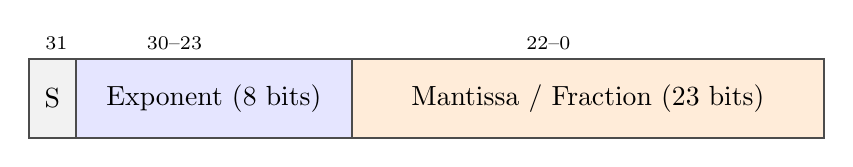
\begin{tikzpicture}[scale=1.0]
  \draw[thick, draw=black!70, fill=gray!10] (-0.1,0) rectangle (0.5,1) node[midway]{S};
  \draw[thick, draw=black!70, fill=blue!10] (0.5,0) rectangle (4,1) node[midway]{Exponent (8 bits)};
  \draw[thick, draw=black!70, fill=orange!15] (4,0) rectangle (10,1) node[midway]{Mantissa / Fraction (23 bits)};
  \node[above] at (0.25,1) {\scriptsize 31};
  \node[above] at (1.75,1) {\scriptsize 30--23};
  \node[above] at (6.5,1) {\scriptsize 22--0};
\end{tikzpicture}
\end{center}
with the sign bit $S$, an 8-bit biased exponent $E$, and a 23-bit
fraction $f = b_1 b_2 \cdots b_{23}$. The value is
\begin{equation}
x \;=\; (-1)^{S} \,\cdot\, 2^{E - 127} \,\cdot\,
\left(1 + \sum_{i=1}^{23} b_i\, 2^{-i}\right).
\label{eq:fp32}
\end{equation}
The leading ``$1+$'' is the \emph{hidden bit}: for a normalised number,
the leading significand bit is always $1$ and so need not be stored,
buying one extra bit of precision for free. The bias of $127$ allows
$E - 127$ to range over negative and positive values symmetrically.

\begin{example}[Decoding $0.15625$]
The bit pattern
\texttt{0\,\,01111100\,\,01000000000000000000000} decodes as
\[
x = (-1)^0 \cdot 2^{124-127} \cdot \left(1 + \tfrac{1}{4}\right)
  = \tfrac{1}{8} \cdot \tfrac{5}{4} = 0.15625.
\]
\end{example}

\subsection{Special values}

Certain bit patterns are reserved for non-numeric results:
\begin{itemize}[leftmargin=1.5em, itemsep=2pt]
    \item \textbf{$\pm 0$}: exponent and fraction both zero.
    \item \textbf{$\pm\infty$}: all exponent bits set, fraction zero.
          Produced by overflow or by $1/0$.
    \item \textbf{NaN} (\emph{Not a Number}): all exponent bits set,
          fraction nonzero. Produced by indeterminate operations such as
          $0/0$ or $\infty - \infty$.
    \item \textbf{Subnormals}: exponent bits zero, fraction nonzero,
          representing values smaller than the smallest normalised number
          at the cost of reduced precision.
\end{itemize}

A common confusion: \texttt{NaN} is not ``uninitialised memory'' or ``a
null pointer''. It is a first-class, fully encoded floating-point value,
specifically designed so that any arithmetic operation involving it
yields \texttt{NaN}. Once a \texttt{NaN} appears in a weight tensor, it
tends to propagate across a forward pass and contaminate the whole
model---a failure mode we shall return to.

\subsection{Why lower precision?}

The rationale for using fewer than $32$ bits per number is threefold.

\begin{enumerate}[leftmargin=1.8em, itemsep=2pt]
    \item \textbf{Memory footprint.} Halving the bits halves the storage
          for weights, gradients, activations, and optimizer state. This
          matters enormously in embedded settings and in large-model
          training, where memory is the binding constraint.
    \item \textbf{Arithmetic throughput.} Modern accelerators can perform
          more low-precision operations per cycle than high-precision
          ones, sometimes by factors of $8$--$16$.
    \item \textbf{Bandwidth.} Less data per number means less traffic
          over memory buses and network links---often the dominant cost
          in distributed settings.
\end{enumerate}

Specialised hardware (Tensor Cores, TPU matrix units) amplifies these
gains beyond a naive linear scaling: the speedups are frequently
\emph{superlinear} in the reduction of bit width.

\subsection{The zoo of formats}

We now survey the formats in contemporary use. Each is a point in the
design space defined by the allocation of bits between sign, exponent
(range), and mantissa (precision). The comparison of FP32, TF32, FP16, and
BF16 follows NVIDIA's blog post
\href{https://developer.nvidia.com/blog/accelerating-ai-training-with-tf32-tensor-cores/}{\textit{Accelerating
AI Training with NVIDIA TF32 Tensor Cores}}.

\begin{center}
\renewcommand{\arraystretch}{1.25}
\setlength{\tabcolsep}{4pt}
\small
\begin{tabular}{@{}lcccl@{}}
\toprule
\textbf{Format} & \textbf{Sign} & \textbf{Exponent (range)} &
\textbf{Mantissa (precision)} & \textbf{Notes} \\
\midrule
FP32 & 1 & 8 & 23 & IEEE 754 single precision \\
TF32 & 1 & 8 & 10 & NVIDIA Ampere internal type \\
FP16 & 1 & 5 & 10 & IEEE 754 half precision \\
BF16 & 1 & 8 & 7 & Google Brain float \\
FP8 E4M3 & 1 & 4 & 3 & For weights/activations \\
FP8 E5M2 & 1 & 5 & 2 & For gradients \\
\bottomrule
\end{tabular}
\par\smallskip
{\small Allocation of bits across common floating-point formats.}
\end{center}

Several design choices are worth teasing apart.

\begin{description}[leftmargin=1.5em, style=nextline]
    \item[FP16 vs.\ BF16.] Both use $16$ bits, but they make opposite
        trade-offs. FP16 inherits $5$ exponent bits from IEEE 754 half
        precision; its dynamic range is accordingly narrow, and
        underflow to zero is a real hazard during training. BF16 keeps
        FP32's $8$-bit exponent, matching its range, at the cost of a
        miserly $7$-bit mantissa. In deep learning, where gradient
        magnitudes span many orders of magnitude but precision
        requirements are modest, BF16's trade-off is usually the right
        one---and it is the format behind most large-model training on
        H100 hardware today. (BF16 is available on CPUs, TPUs, and recent
        GPUs; see the
        \href{http://pytorch.org/xla/release/1.9/index.html\#xla-tensors-and-bfloat16}{PyTorch/XLA
        documentation on BF16}. In PyTorch it is one call away:
        \texttt{Tensor.bfloat16()}.)
    \item[TF32.] TensorFloat-32 is a peculiar beast. It is not a storage
        format; tensors in memory remain in FP32. Rather, when Tensor
        Cores on Ampere (or newer) hardware perform a matrix
        multiplication, they internally round operands to a TF32-like
        format ($8$-bit exponent, $10$-bit mantissa), multiply, and
        \emph{accumulate in FP32}. The output is returned in full FP32.
        This delivers most of the speedup of lower precision with minimal
        impact on accuracy, and requires no code changes. PyTorch enabled
        TF32 by default for much of its history, then disabled it by
        default in later versions to restore bit-exact reproducibility;
        it remains trivially toggleable. TF32 is never exposed as a data
        type, only as a mode for specific operations---the NVIDIA post
        linked above explains the mechanism in detail.
\end{description}

\begin{center}
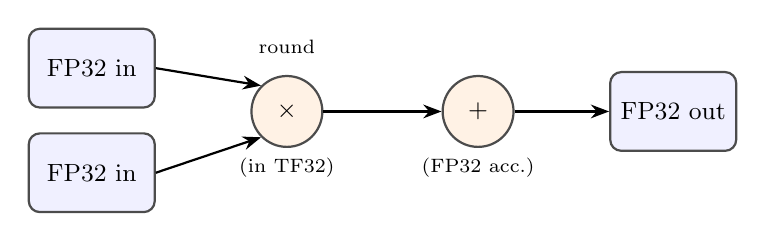
\begin{tikzpicture}[
    node distance=1.4cm,
    box/.style={rectangle, rounded corners, draw=black!70, thick,
                minimum height=1cm, minimum width=1.6cm, font=\small,
                fill=blue!6},
    op/.style={circle, draw=black!70, thick, minimum size=0.9cm,
               font=\small, fill=orange!10},
    arr/.style={-Stealth, thick}
]
\node[box] (in1) {FP32 in};
\node[box, below=0.3cm of in1] (in2) {FP32 in};
\node[op, right=1.2cm of in1, yshift=-0.55cm] (mul) {$\times$};
\node[font=\scriptsize, below=0pt of mul] {(in TF32)};
\node[op, right=1.5cm of mul] (add) {$+$};
\node[font=\scriptsize, below=0pt of add] {(FP32 acc.)};
\node[box, right=1.2cm of add] (out) {FP32 out};

\draw[arr] (in1.east) -- (mul.north west);
\draw[arr] (in2.east) -- (mul.south west);
\draw[arr] (mul) -- (add);
\draw[arr] (add) -- (out);

\node[above=0.15cm of mul, font=\scriptsize, align=center] {round};
\end{tikzpicture}
\par\smallskip
{\small Tensor Core multiply-add on TF32: operands are rounded to reduced
precision for the multiply, but accumulation and the final output remain
in FP32.}
\end{center}

\begin{description}[leftmargin=1.5em, style=nextline]
    \item[FP8 (E4M3 and E5M2).] With the H100 generation, NVIDIA
        introduced native $8$-bit floating-point. Two variants are
        provided because different tensors have different needs:
        \begin{itemize}[leftmargin=1.5em, itemsep=2pt]
            \item \textbf{E4M3} ($4$-bit exponent, $3$-bit mantissa):
                  higher precision, narrower range. Used for
                  \emph{weights and activations}, which benefit from
                  precision and whose distributions are relatively
                  well-behaved.
            \item \textbf{E5M2} ($5$-bit exponent, $2$-bit mantissa):
                  wider range, lower precision. Used for
                  \emph{gradients}, whose magnitudes can span many
                  orders of magnitude and for which overflow is
                  catastrophic.
        \end{itemize}
\end{description}

Native $8$-bit representation on its own is insufficient for stable
training---the dynamic range is simply too narrow. FP8 training works
only with \emph{scaling}, which we address next. (The two formats are
described in Micikevicius et al., \emph{FP8 Formats for Deep Learning},
2022.)

%%%%%%%%%%%%%%%%%%%%%%%%%%%%%%%%%%%%%%%%%%%%%%%%%%%%%%%%%%%%%%%%%%%%%%%%
\section{Tensor Cores and Hardware Alignment}
%%%%%%%%%%%%%%%%%%%%%%%%%%%%%%%%%%%%%%%%%%%%%%%%%%%%%%%%%%%%%%%%%%%%%%%%

Tensor Cores, introduced with the Volta architecture in 2017 and refined
in every generation since, are specialised functional units that
accelerate the matrix multiply-accumulate
\begin{equation}
D = A \cdot B + C
\end{equation}
at low precision. An apt mental model is that they are
FPGAs-within-the-GPU: fixed-function blocks dedicated exclusively to MMA
operations, delivering claimed speedups of $8$--$16\times$ over the
general-purpose CUDA cores for suitable workloads.

\subsection{Conditions for Tensor Core utilisation}

Tensor Cores are not engaged automatically for every matrix
multiplication. Two conditions must hold: the hardware and CUDA libraries
must support the precision in use, and the matrix dimensions must be
compatible with the hardware's tile size. With older libraries, misaligned
dimensions disable Tensor Cores outright; with recent ones they remain
usable but run far below peak. The specific requirements vary by
precision:

\begin{center}
\renewcommand{\arraystretch}{1.25}
\begin{tabular}{@{}lp{3.3cm}p{7.3cm}@{}}
\toprule
\textbf{Precision} & \textbf{cuBLAS $<11.0$, cuDNN $<7.6.3$} &
\textbf{cuBLAS $\geq 11.0$, cuDNN $\geq 7.6.3$} \\
\midrule
INT8 & multiples of 16 &
  always usable, but most efficient with multiples of 16; on A100,
  multiples of 128 \\
FP16 & multiples of 8 &
  always usable, but most efficient with multiples of 8; on A100,
  multiples of 64 \\
TF32 & N/A &
  always usable, but most efficient with multiples of 4; on A100,
  multiples of 32 \\
FP64 & N/A &
  always usable, but most efficient with multiples of 2; on A100,
  multiples of 16 \\
\bottomrule
\end{tabular}
\par\smallskip
{\small Tensor Core requirements by cuBLAS and cuDNN version for common
data precisions. The requirements apply to the matrix dimensions $M$,
$N$, and $K$. The table is from NVIDIA's
\href{https://docs.nvidia.com/deeplearning/performance/dl-performance-matrix-multiplication/index.html\#requirements-tc}{matrix
multiplication performance guide}; see also the GTC 2019 talk
\href{https://developer.download.nvidia.com/video/gputechconf/gtc/2019/presentation/s9926-tensor-core-performance-the-ultimate-guide.pdf}{\textit{Tensor
Core Performance: The Ultimate Guide}}.}
\end{center}

\subsection{The padding cliff}

The dimensional constraints bite hard in practice. Consider a projection
layer from $1024$ to $V$, where $V$ is a vocabulary size. If $V = 33708$,
no luck---the number is not a multiple of $8$, and the Tensor Cores
cannot be used at full efficiency. Bumping $V$ to $33712$ (adding four
unused output positions!) can increase throughput several-fold, because
the hardware can now tile the operation cleanly. (The measurements behind
this example are from the two NVIDIA sources cited above.)

The lesson is subtle: \emph{what looks like an innocent architectural
hyperparameter can determine whether your matmul runs at $25$~TFLOPS or
$85$~TFLOPS}. It is standard practice to pad vocabularies and hidden
dimensions to friendly multiples. For feed-forward layers, which already
operate on large batches of well-aligned dimensions, throughput is
usually saturated and less sensitive to these choices.

\begin{remark}[Verification]
The NVIDIA profiler can confirm whether your matrix multiplications are
actually dispatched to Tensor Cores or have fallen back to vanilla CUDA
cores. \emph{Trust, but verify.}
\end{remark}

%%%%%%%%%%%%%%%%%%%%%%%%%%%%%%%%%%%%%%%%%%%%%%%%%%%%%%%%%%%%%%%%%%%%%%%%
\section{Mixed Precision Training}
\label{sec:amp}
%%%%%%%%%%%%%%%%%%%%%%%%%%%%%%%%%%%%%%%%%%%%%%%%%%%%%%%%%%%%%%%%%%%%%%%%

\subsection{The case against pure FP16}

Training a network entirely in FP16 does not work. Or, more precisely:
matrix multiplications work fine in FP16, because Tensor Cores handle
them natively and the accumulator is in FP32. But other operations---the
softmax at the output of attention, batch normalisation, loss
computation---involve sums, exponentials, and divisions that genuinely
require FP32's dynamic range to avoid overflow, underflow, or
catastrophic precision loss.

\subsection{Automatic Mixed Precision}

Automatic Mixed Precision (AMP), exposed in PyTorch via
\texttt{torch.cuda.amp}, resolves this by \emph{casting per operation}. A
rough mental model of the forward pass:
\begin{center}
\texttt{Input} $\to$ \texttt{Conv (FP16)} $\to$ \texttt{ReLU (FP16)}
$\to$ \texttt{BatchNorm (FP32)} $\to$ \texttt{Loss (FP32)}.
\end{center}
Operations on an internal ``allow list'' (matrix multiplications,
convolutions) run in FP16 or BF16; operations on a ``deny list''
(reductions, softmaxes, batch norm statistics) run in FP32; operations in
between follow the precision of their inputs. AMP is not strictly
CUDA-specific---analogous machinery exists for other accelerators.

\subsection{The precision-underflow problem}

\begin{proposition}[Why naive FP16 updates disappear]
Let $w$ be a weight stored in FP16 and $g$ its gradient. If
\[
|\eta\, g| \;<\; \epsilon\, |w|
\]
where $\eta$ is the learning rate and $\epsilon$ is the relative
precision of FP16 ($\approx 10^{-3}$), then the update
$w \gets w - \eta g$ is indistinguishable from $w$ in the FP16
representation: the update is silently dropped, and training stalls.
\end{proposition}

This is not hypothetical; late in training, when weights are large and
gradients small, it is the common case. The remedy is to maintain a
\emph{master copy} of the weights in FP32 and apply all updates there,
casting back to FP16 only for the next forward pass.


\subsection{Master weights and loss scaling}

Master weights solve the problem on the update side. A related hazard
lives on the gradient side: very small gradient values can underflow to
zero in FP16. The standard remedy is \emph{loss scaling}: multiply the
loss by a constant factor before the backward pass, which (by the chain
rule) scales every gradient by the same factor and lifts it into FP16's
representable range; then divide the factor out again, in FP32, before
clipping and before the optimizer update. The diagram below shows one full
training step.

\begin{center}
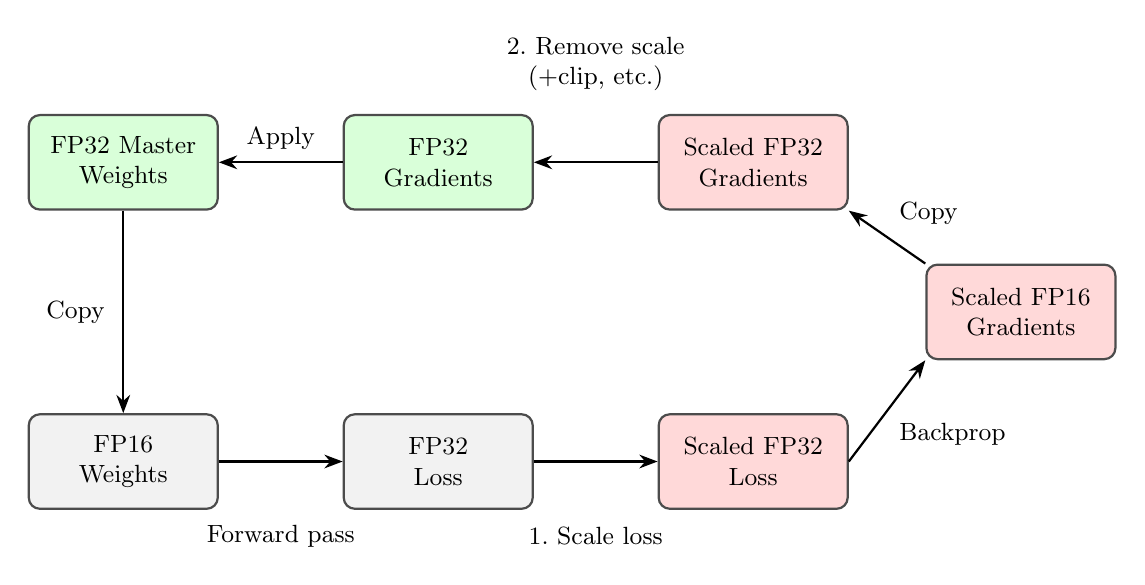
\begin{tikzpicture}[
    box/.style={rectangle, rounded corners, draw=black!70, thick,
                minimum width=2.4cm, minimum height=1.2cm, align=center,
                font=\small},
    master/.style={box, fill=green!15},
    plain/.style={box, fill=gray!10},
    scaled/.style={box, fill=red!15},
    arr/.style={-Stealth, thick},
    lab/.style={font=\small}
]
  % top row: FP32 master weights, FP32 gradients, scaled FP32 gradients
  \node[master] (mw)   at (0,0)    {FP32 Master\\Weights};
  \node[master] (g32)  at (4,0)    {FP32\\Gradients};
  \node[scaled] (sg32) at (8,0)    {Scaled FP32\\Gradients};
  % right: scaled FP16 gradients
  \node[scaled] (sg16) at (11.4,-1.9) {Scaled FP16\\Gradients};
  % bottom row: FP16 weights, FP32 loss, scaled FP32 loss
  \node[plain]  (w16)  at (0,-3.8) {FP16\\Weights};
  \node[plain]  (l32)  at (4,-3.8) {FP32\\Loss};
  \node[scaled] (sl)   at (8,-3.8) {Scaled FP32\\Loss};

  \draw[arr] (sg32) -- (g32);
  \draw[arr] (g32)  -- node[lab, above=1pt] {Apply} (mw);
  \draw[arr] (mw)   -- node[lab, left=3pt]   {Copy}  (w16);
  \draw[arr] (w16)  -- (l32);
  \draw[arr] (l32)  -- (sl);
  \draw[arr] (sl.east) -- node[lab, below right=1pt] {Backprop} (sg16.south west);
  \draw[arr] (sg16.north west) -- node[lab, above right=1pt] {Copy} (sg32.south east);

  \node[lab, align=center] at (6,1.25) {2.\ Remove scale\\(+clip, etc.)};
  \node[lab] at (2,-4.75) {Forward pass};
  \node[lab] at (6,-4.75) {1.\ Scale loss};
\end{tikzpicture}
\par\smallskip
{\small One step of mixed-precision training with FP32 master weights and
loss scaling. Green: FP32 master state; grey: FP16 weights and FP32 loss;
red: scaled quantities. The illustration from NVIDIA's
\href{https://nvlabs.github.io/eccv2020-mixed-precision-tutorial/files/dusan_stosic-training-neural-networks-with-tensor-cores.pdf}{ECCV
2020 mixed-precision tutorial}.}
\end{center}

Reading the diagram clockwise from the master weights:
\begin{enumerate}[leftmargin=1.8em, itemsep=2pt]
    \item \textbf{Copy} the FP32 master weights to an FP16 working copy.
    \item \textbf{Forward pass} in FP16, producing an FP32 loss.
    \item \textbf{Scale the loss}, then \textbf{backpropagate}: the
          gradients come out scaled and in FP16.
    \item \textbf{Copy} the scaled gradients to FP32.
    \item \textbf{Remove the scale} (and clip, etc.), leaving the true FP32
          gradients.
    \item \textbf{Apply} the update to the FP32 master weights.
\end{enumerate}

\subsection{Memory accounting for Adam}

The Adam optimizer maintains, per parameter, the parameter value itself
plus two running statistics: the first moment $\hat{m}$ (an exponential
moving average of the gradient) and the second moment $\hat{v}$ (of the
squared gradient). We track, in addition, the gradient itself during the
backward pass. Tallying the bytes per parameter under standard FP32
training and under AMP with the master-weight trick:

\begin{center}
\renewcommand{\arraystretch}{1.25}
\begin{tabular}{@{}lcc@{}}
\toprule
\textbf{Quantity} & \textbf{Standard FP32} & \textbf{AMP (master weights)} \\
\midrule
Parameter (working copy)  & 4 bytes (FP32) & 2 bytes (FP16) \\
Gradient                  & 4 bytes (FP32) & 2 bytes (FP16; sometimes 4) \\
Master parameter          & ---            & 4 bytes (FP32) \\
First moment $\hat{m}$    & 4 bytes (FP32) & 4 bytes (FP32) \\
Second moment $\hat{v}$   & 4 bytes (FP32) & 4 bytes (FP32) \\
\midrule
\textbf{Total}            & \textbf{16 bytes per parameter} &
                            \textbf{16 bytes per parameter} \\
\bottomrule
\end{tabular}
\par\smallskip
{\small Memory per parameter for Adam under standard and mixed-precision
training.}
\end{center}

A $1$~billion-parameter model therefore costs $16$~GB for weights,
gradients, and optimizer state alone, before activations. (If gradients are
kept in FP32 under AMP, which some implementations do, the AMP column rises
to $18$~bytes.)

\begin{aside}[The surprising arithmetic of AMP]
The striking observation, often missed by newcomers, is that AMP
\emph{does not reduce the per-parameter memory footprint of the
weights-plus-optimizer-state bundle}. We simply shuffle bytes: we save
$2$~bytes per parameter by moving the working copy to FP16, then spend
$4$~bytes storing the FP32 master copy. Where, then, does the memory
advantage come from?
\end{aside}

\subsection{The real prize: activation memory}

The answer is \emph{activations}. During the forward pass, the values
produced by each layer must be retained until the backward pass computes
gradients through them. For a deep network with long sequences or large
images, activation memory dominates the footprint---often exceeding
weights by an order of magnitude.

By running the forward pass in FP16 or BF16, AMP halves the storage for
these intermediate tensors. This is the dominant source of memory
savings, and it is what lets practitioners double their batch size or
double their model depth on the same hardware.

There are also secondary costs: casts between FP16 and FP32 consume a
small amount of time and occasionally materialise additional tensors, and
the backward pass, which manages a mix of precisions, can be slightly
more expensive than the forward. These overheads are real but generally
dwarfed by the gains.

%%%%%%%%%%%%%%%%%%%%%%%%%%%%%%%%%%%%%%%%%%%%%%%%%%%%%%%%%%%%%%%%%%%%%%%%
\section{FP8 Training and Scaled Representations}
%%%%%%%%%%%%%%%%%%%%%%%%%%%%%%%%%%%%%%%%%%%%%%%%%%%%%%%%%%%%%%%%%%%%%%%%

FP8 training, now feasible on H100-class accelerators, pushes the
precision reduction further. But an FP8 value in isolation cannot
represent the dynamic range typical of deep learning tensors: with only
$4$ or $5$ exponent bits, we cover perhaps $10^{10}$ at best, whereas
gradient magnitudes in a large Transformer routinely span $10^{20}$ or
more. Raw casting fails.

\subsection{Scaling as a first-class citizen}

The remedy is to attach a \emph{scale factor} to the tensor. A value is
represented as the pair $(D, S)$, where $D$ is the FP8 data and $S$ is
the (higher-precision) scale:
\begin{equation}
v \;=\; S \cdot D.
\end{equation}
For matrix multiplication of two scaled tensors $A = (D_A, S_A)$ and
$B = (D_B, S_B)$, the hardware computes
\begin{equation}
C \;=\; A B \;=\; (S_A S_B) \cdot (D_A D_B),
\end{equation}
multiplying the FP8 payloads and folding the scales into a separate
higher-precision factor. The scales never need to participate in the
per-element arithmetic; they modulate the result once the multiplication
is complete.

\subsection{Granularity: FP8 vs.\ MXFP8}

A single scale for an entire tensor is often too coarse. If one corner of
a tensor has large values and another has small ones, a global scale fits
neither: it will either overflow the large values or underflow the small.
\emph{Microscaling} formats (MXFP8) partition the tensor into small
blocks---typically $32$ elements---and assign each block its own scale.

\begin{center}
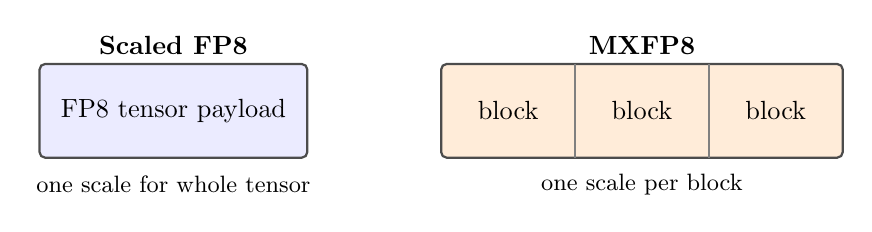
\begin{tikzpicture}[scale=0.85, every node/.style={scale=0.95}]
  % Tensor-level scaled FP8
  \draw[thick, draw=black!70, rounded corners=2pt, fill=blue!8] (0,0) rectangle (4,1.4);
  \node[align=center] at (2,0.7) {FP8 tensor payload};
  \node at (2,-0.4) {\small one scale for whole tensor};
  \node[above] at (2,1.4) {\textbf{Scaled FP8}};

  % MXFP8
  \draw[thick, draw=black!70, rounded corners=2pt, fill=orange!15] (6,0) rectangle (12,1.4);
  \foreach \x in {8,10} {
    \draw[thick, black!50] (\x,0) -- (\x,1.4);
  }
  \node at (7,0.7) {block};
  \node at (9,0.7) {block};
  \node at (11,0.7) {block};
  \node at (9,-0.4) {\small one scale per block};
  \node[above] at (9,1.4) {\textbf{MXFP8}};
\end{tikzpicture}
\par\smallskip
{\small Scaled FP8 uses a single scale per tensor; MXFP8 (microscaling)
partitions the tensor into blocks and gives each its own scale.}
\end{center}

Without per-block scaling, FP8 training tends to collapse after a small
number of iterations---one pathological block with the wrong scale
suffices to corrupt the entire gradient. MXFP8, by adapting to local
statistics, is dramatically more robust.

\begin{remark}[Reference implementations]
For practical implementations, consult NVIDIA's TransformerEngine
(\href{https://github.com/NVIDIA/TransformerEngine}{\texttt{github.com/NVIDIA/TransformerEngine}})
and PyTorch's \texttt{torchao} library
(\href{https://github.com/pytorch/ao/tree/main/torchao/float8}{\texttt{torchao/float8}}).
Both handle the bookkeeping of scales, casts, and fused kernels that make
FP8 training stable in practice.
\end{remark}

%%%%%%%%%%%%%%%%%%%%%%%%%%%%%%%%%%%%%%%%%%%%%%%%%%%%%%%%%%%%%%%%%%%%%%%%
\section{Data Loading and Storage}
%%%%%%%%%%%%%%%%%%%%%%%%%%%%%%%%%%%%%%%%%%%%%%%%%%%%%%%%%%%%%%%%%%%%%%%%

\subsection{The latency hierarchy}

Before optimizing a data pipeline, internalise the orders of magnitude at
play. The following numbers (approximate, circa modern hardware; the
famous ``Latency Numbers Every Programmer Should Know'' by Dean and
Norvig) reveal why the choice of storage medium matters so much. See the
\href{https://colin-scott.github.io/personal_website/research/interactive_latency.html}{interactive
version} of this table, which lets one slide the year from 2000 to 2020
and watch each entry shrink.

\begin{center}
\renewcommand{\arraystretch}{1.25}
\begin{tabular}{@{}lr@{}}
\toprule
\textbf{Operation} & \textbf{Latency} \\
\midrule
L1 cache reference & $\sim\!1$ ns \\
Branch misprediction & $\sim\!3$ ns \\
L2 cache reference & $\sim\!4$ ns \\
Mutex lock/unlock & $\sim\!17$ ns \\
Main memory reference & $\sim\!100$ ns \\
Compress 1 KB with Snappy & $\sim\!2$ $\mu$s \\
Send 2 KB over commodity network & $\sim\!44$ ns \\
Read 1 MB sequentially from memory & $\sim\!3$ $\mu$s \\
SSD random read & $\sim\!16$ $\mu$s \\
Read 1 MB sequentially from SSD & $\sim\!49$ $\mu$s \\
Round-trip within a datacentre & $\sim\!0.5$ ms \\
Disk seek & $\sim\!2$ ms \\
Read 1 MB sequentially from disk & $\sim\!825$ $\mu$s \\
Packet round-trip, California~$\to$~Netherlands & $\sim\!150$ ms \\
\bottomrule
\end{tabular}
\par\smallskip
{\small Typical latencies across the storage hierarchy.}
\end{center}

The gap between L1 cache and a transcontinental packet is eight orders of
magnitude. Any data-loading architecture that fails to respect this
hierarchy---for example, by issuing synchronous reads from spinning disk
in the critical path of the training loop---will spend nearly all of its
time waiting.

\subsection{Two design questions}

Data pipeline design reduces to two questions:

\begin{enumerate}[leftmargin=1.8em, itemsep=2pt]
    \item \textbf{What to read?} Which storage format?
    \item \textbf{How to read?} Which execution strategy?
\end{enumerate}

\subsubsection*{What to read: storage formats}

Raw files (JPEGs, WAVs, text files) have a single virtue: they are
directly inspectable, which is priceless during data curation. For
training, they are almost always the wrong choice.

\begin{itemize}[leftmargin=1.5em, itemsep=2pt]
    \item \textbf{Binary columnar formats} (Parquet, Arrow) provide
          compact storage, efficient selective reads, and fast
          deserialisation.
    \item \textbf{Record-sequential formats} (TFRecord, WebDataset) store
          many examples in a few large files, reducing filesystem
          overhead and enabling sequential I/O (the fastest kind).
    \item \textbf{Serialisation protocols} (Protobuf, MessagePack) trade
          a little compactness for explicit schemas and cross-language
          compatibility.
\end{itemize}

For specific modalities:
\begin{itemize}[leftmargin=1.5em, itemsep=2pt]
    \item \textbf{Images}: perform heavy, deterministic preprocessing
          ahead of time (resizing, cropping to canonical size,
          colour-space conversion). Leave only stochastic augmentation
          for training time.
    \item \textbf{Text}: tokenize once, offline. Store integer token IDs,
          not Unicode strings. This reduces storage several-fold and
          exactly matches the model's input format, eliminating runtime
          conversion.
    \item \textbf{Audio}: consider compressed formats (FLAC losslessly;
          MP3 or Opus lossily) rather than raw WAV. The perceptual losses
          of lossy codecs are often invisible to model accuracy and can
          shrink storage by an order of magnitude.
\end{itemize}

\subsubsection*{How to read: parallelism and asynchrony}

The principle is straightforward: the GPU must never wait for data. While
the GPU processes batch $n$, the CPU should be preparing batch $n+1$.
PyTorch's \texttt{DataLoader} implements this with worker processes: each
worker reads, decodes, and augments examples in parallel, then hands them
to the main process via shared memory.

Getting this right requires some care. Too few workers and the GPU
stalls; too many and workers contend for CPU and I/O. The number of
workers should roughly match the available CPU cores, and should be tuned
empirically by profiling.

\subsection{Image loading, in particular}

The default Python image loader, \texttt{PIL.Image.open}, is surprisingly
slow.
\begin{itemize}[leftmargin=1.5em, itemsep=2pt]
    \item Use \textbf{Pillow-SIMD}, a drop-in replacement exploiting SIMD
          instructions.
    \item Use better JPEG decoders---\texttt{jpegturbo} on CPU,
          \texttt{nvJPEG} on GPU.
    \item \textbf{Move augmentations to the GPU} when they are expensive.
          Libraries like \emph{Kornia} and \emph{DALI} (NVIDIA Data
          Loading Library) offload the augmentation pipeline to the
          accelerator, where parallelism is abundant and the CPU ceases
          to be the bottleneck.
\end{itemize}

\subsection{Sequence processing: the padding problem}

A batch of sequences must be a rectangular tensor, which forces the
shorter sequences to be padded to the length of the longest. If one pads
naively to the global maximum length across the whole dataset, an
enormous amount of computation is wasted on padding tokens, most of which
contribute nothing to the loss.

The remedy is \emph{dynamic batching}:
\begin{enumerate}[leftmargin=1.8em, itemsep=2pt]
    \item Store sequences \emph{unpadded} on disk.
    \item In the \texttt{collate\_fn}, pad only to the longest sequence
          \emph{in the current batch}.
    \item For further efficiency, \emph{bucket} sequences of similar
          length together so that batches are homogeneous.
    \item For the most aggressive optimisation, \emph{pack} multiple
          short sequences into a single long sequence separated by
          delimiters, eliminating padding almost entirely.
\end{enumerate}

\begin{remark}[A statistical caveat]
Bucketing means that, within an epoch, examples are no longer
independently and identically distributed---the batches are stratified by
length. This violates an assumption of stochastic gradient theory. In
practice, with large datasets and sufficient shuffling within buckets, the
effect on training dynamics is typically negligible; but the reader should
know that it is a trade.
\end{remark}

%%%%%%%%%%%%%%%%%%%%%%%%%%%%%%%%%%%%%%%%%%%%%%%%%%%%%%%%%%%%%%%%%%%%%%%%
\section{Profiling}
\label{sec:profiling}
%%%%%%%%%%%%%%%%%%%%%%%%%%%%%%%%%%%%%%%%%%%%%%%%%%%%%%%%%%%%%%%%%%%%%%%%

\subsection{Benchmarking vs.\ profiling}

\begin{definition}[Benchmarking]
A \emph{black-box} measurement of a program's observable outputs---typically
total execution time---under controlled conditions. Benchmarking answers
the question \emph{did it get faster?}
\end{definition}

\begin{definition}[Profiling]
A \emph{white-box} measurement of a program's internal execution---which
functions were called, how long they ran, how much memory they allocated.
Profiling answers the question \emph{where did the time go?}
\end{definition}

A medical metaphor is clarifying: benchmarking tells you the patient is
still ill; profiling tells you where it hurts. An optimisation campaign
that relies only on benchmarks is flying blind: you can tell you have
changed something, but not whether the change addressed the actual
bottleneck or merely happened to coincide with random timing variation.

\subsection{Python-level profiling}

Several tools cover the Python side:

\begin{itemize}[leftmargin=1.5em, itemsep=2pt]
    \item \textbf{\href{https://docs.python.org/3/library/profile.html\#module-cProfile}{\texttt{cProfile}}}:
          the standard library's deterministic profiler. Records every
          function entry and exit, yielding exact call counts and
          cumulative times. The overhead is nontrivial, which can distort
          the measurements it is meant to make.
    \item \textbf{\href{https://github.com/plasma-umass/scalene}{\texttt{scalene}}}:
          a modern sampling profiler that reports CPU, GPU, and memory
          usage separately, with very low overhead.
    \item \textbf{\href{https://github.com/benfred/py-spy}{\texttt{py-spy}}}:
          a sampling profiler that can \emph{attach to a running process}
          without restarting it. Essential for diagnosing production
          issues.
\end{itemize}

\subsection{GPU profiling}

For the GPU, Python-level tools are insufficient; one must instrument the
CUDA runtime.

\begin{itemize}[leftmargin=1.5em, itemsep=2pt]
    \item \textbf{Nsight Systems}: a \emph{system-wide} profiler. Records
          a timeline of CPU threads, GPU kernels, API calls, and
          synchronisation events. This is the tool for understanding the
          orchestration of a training step---where waits occur, where
          overlap fails, how data movement interleaves with computation.
    \item \textbf{Nsight Compute}: a \emph{kernel-level} profiler.
          Answers questions like: what is the occupancy of this kernel?
          Is it memory-bound or compute-bound? What fraction of Tensor
          Core capacity is it using? Indispensable when you are writing
          or tuning a specific kernel.
\end{itemize}

The division of labour is clean: \textbf{Nsight Systems} shows you
\emph{which} kernel is your problem; \textbf{Nsight Compute} shows you
\emph{why}. The Nsight timeline is from the GTC
2019 talk
\href{https://developer.download.nvidia.com/video/gputechconf/gtc/2019/presentation/s9339-profiling-deep-learning-networks.pdf}{\textit{Profiling
Deep Learning Networks}}.

Inside PyTorch, the modern instrumentation is
\href{https://pytorch.org/docs/stable/profiler.html\#module-torch.profiler}{\texttt{torch.profiler}},
which wraps a region of code in a context manager and emits a structured
trace (viewable in Chrome's tracing tool, TensorBoard, or Perfetto); the
official
\href{https://pytorch.org/tutorials/recipes/recipes/profiler_recipe.html}{profiler
recipe} is the best place to start.

\subsection{Recognising performance patterns}

Profiling traces reveal recurring patterns. Two are fundamental. (The
patterns, and the Nsight Systems traces are from Paul Bridger's post
\href{https://paulbridger.com/posts/nsight-systems-systematic-optimization/}{\textit{Nsight
Systems: Systematic Optimization}}.)

\subsubsection*{Pattern 1: GPU compute-bound}

The host CPU enqueues operations into the command queue faster than the
device GPU can execute them. The queue stays full; the GPU is never idle;
the CPU ends up waiting at a synchronisation point for the last operation
to complete.

\begin{center}
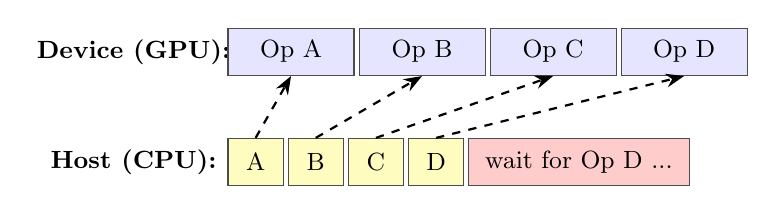
\begin{tikzpicture}[
    node distance=0.1cm,
    op/.style={rectangle, draw=black!70, minimum width=1.2cm,
               minimum height=0.6cm, font=\small},
    arr/.style={-Stealth, thick}
]
  % Device row
  \node[font=\small] at (-2,0) {\textbf{Device (GPU):}};
  \node[op, fill=blue!10, minimum width=1.6cm] (dA) at (0,0) {Op A};
  \node[op, fill=blue!10, right=0.05cm of dA, minimum width=1.6cm] (dB) {Op B};
  \node[op, fill=blue!10, right=0.05cm of dB, minimum width=1.6cm] (dC) {Op C};
  \node[op, fill=blue!10, right=0.05cm of dC, minimum width=1.6cm] (dD) {Op D};

  % Host row
  \node[font=\small] at (-2,-1.4) {\textbf{Host (CPU):}};
  \node[op, fill=yellow!25, minimum width=0.7cm] (hA) at (-0.45, -1.4) {A};
  \node[op, fill=yellow!25, right=0.05cm of hA, minimum width=0.7cm] (hB) {B};
  \node[op, fill=yellow!25, right=0.05cm of hB, minimum width=0.7cm] (hC) {C};
  \node[op, fill=yellow!25, right=0.05cm of hC, minimum width=0.7cm] (hD) {D};
  \node[op, fill=red!20, right=0.05cm of hD, minimum width=2.8cm] (sync) {wait for Op D ...};

  % Arrows host-to-device
  \foreach \src/\dst in {hA/dA, hB/dB, hC/dC, hD/dD} {
    \draw[arr, dashed] (\src.north) -- (\dst.south);
  }
\end{tikzpicture}
\par\smallskip
{\small Compute-bound pattern: the GPU is saturated. The host finishes
dispatching quickly and waits.}
\end{center}

This is the \emph{best-case scenario}. The GPU is the bottleneck and the
GPU is the most expensive resource; we have done our job. Further gains
require making the model itself cheaper---through lower precision, better
kernels, or algorithmic improvements. There is no point
micro-optimising the Python side.

\subsubsection*{Pattern 2: CPU / CUDA-API-bound}

The GPU is faster than the CPU can feed it. Between kernel executions, the
device sits idle waiting for the next dispatch.

\begin{center}
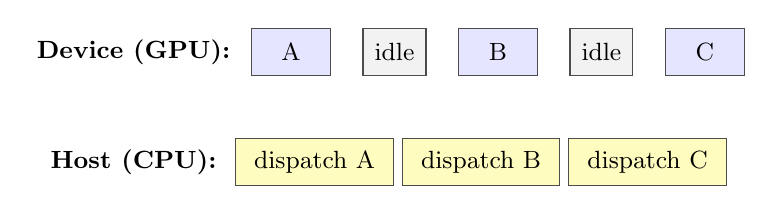
\begin{tikzpicture}[
    op/.style={rectangle, draw=black!70, minimum height=0.6cm, font=\small},
    arr/.style={-Stealth, thick}
]
  % Device row
  \node[font=\small] at (-2,0) {\textbf{Device (GPU):}};
  \node[op, fill=blue!10, minimum width=1cm] (dA) at (0,0) {A};
  \node[op, fill=gray!10, right=0.4cm of dA, minimum width=0.8cm] (id1) {idle};
  \node[op, fill=blue!10, right=0.4cm of id1, minimum width=1cm] (dB) {B};
  \node[op, fill=gray!10, right=0.4cm of dB, minimum width=0.8cm] (id2) {idle};
  \node[op, fill=blue!10, right=0.4cm of id2, minimum width=1cm] (dC) {C};

  % Host row
  \node[font=\small] at (-2,-1.4) {\textbf{Host (CPU):}};
  \node[op, fill=yellow!25, minimum width=2cm] (hA) at (0.3,-1.4) {dispatch A};
  \node[op, fill=yellow!25, right=0.1cm of hA, minimum width=2cm] (hB) {dispatch B};
  \node[op, fill=yellow!25, right=0.1cm of hB, minimum width=2cm] (hC) {dispatch C};
\end{tikzpicture}
\par\smallskip
{\small API-bound pattern: the GPU stalls between kernels because the host
cannot dispatch work quickly enough.}
\end{center}

This is diagnosable and fixable:
\begin{itemize}[leftmargin=1.5em, itemsep=2pt]
    \item \textbf{Reduce dispatch overhead.} Use \texttt{torch.compile} to
          fuse kernels, or CUDA Graphs to record a sequence of operations
          and replay them as a single atomic unit.
    \item \textbf{Increase batch size.} Larger kernels amortise fixed
          dispatch costs over more arithmetic.
    \item \textbf{Eliminate host-device synchronisation.} Every
          \texttt{tensor.item()} or \texttt{tensor.cpu()} in the hot loop
          is a potential disaster, because it forces the device to flush
          and the host to wait.
\end{itemize}

This pattern is especially pernicious in \emph{inference}, where batch
sizes are small and dispatch overhead looms large. It is the pattern CUDA
Graphs were designed to solve.

Profiling traces often reveal frequent interleaving between host and
device activity---a Sync point here, a Sync point there---each one a
micro-stall. The cumulative cost is substantial. The goal is to offload
\emph{long sequences} of work to the GPU at a time, keeping the device
autonomous and the host minimally involved in the inner loop.


\end{document}